\section{Conclusions} 
\label{sec:conclusions}
In this paper we design an architecture to efficiently accelerate S-W, the computation bottleneck in BWA-MEM, the state-of-the-art read aligner. 
Massive task-level parallelism, sharply varied input sizes, and software pruning strategies are emphasized in our design. 
Our FPGA implementation demonstrates about 26.4x speedup compared to a 24-thread Intel Xeon server, as well as up to a 6x improvement over wavefront-based implementations. 

\begin{figure}[!hbt]
	\begin{center}
		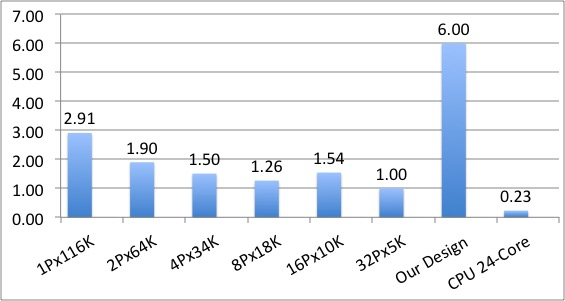
\includegraphics[width=2.5in]{Figures/F2C5.jpg}
		\caption {Performance comparison between our design and a set of wavefront-based designs.}
		\label{fig:F2C5}
	\end{center}
\end{figure}
\vspace{-10pt}

